\newpage
\section{Interakcja z użytkownikiem}
W celu poszerzenia możliwości obsługi akcji użytkownika o zdarzenia myszy do interfejsu \lstinline{IView} opisanego na listingu \ref{lst:iView} dodano metody z listingu \ref{lst:intMethods}.

\begin{lstlisting}[language=C++, caption=Metody interfejsu IView do obsługi zdarzeń myszy., label={lst:intMethods}]
void onMouse(int btn, int state, int x, int y);
void onMotion(GLsizei x, GLsizei y) = 0;
\end{lstlisting}
W ogólnym przypadku metoda \lstinline{onMouse} zapisywała stan, klawisz przycisku myszy i jej pozycję, a metoda \lstinline{onMotion} odpowiadała za wykonywanie akcji odpowiedzialnej za ruch myszy.
\subsection{Perspektywa}
Za wyświetlenie perspektywiczne odpowiada metoda \lstinline{gluPerspective}, która zastąpiła metodę \lstinline{gluOrtho} odpowiedzialną za wyświetlanie ortograficzne w metodzie \lstinline{changeSize}. Widok obserwatora definiuje metoda \lstinline{gluLookAt}, do której poprzez parametry podane zostają pozycje kamery, celu i jej kierunku obrotu. W metodzie \lstinline{render} widoku \lstinline{TeapotView} dodane zostało wywołanie metody \lstinline{gluLookAt}, które argumenty czerpie ze zmiennych klasy widoku, co daje możliwość dowolnego sterowania pozycją obserwatora.
\begin{lstlisting}[language=C++, caption=Definicja i wywołanie metody \lstinline{gluLookAt}., label={lst:intGluLookAt}]
void gluLookAt(
    GLdouble eyeX, GLdouble eyeY, GLdouble eyeZ,
    GLdouble centerX, GLdouble centerY, GLdouble centerZ,
    GLdouble upX, GLdouble upY, GLdouble upZ
);
//---
gluLookAt(
    eye.x + center.x,eye.y + center.y, eye.z + center.z,
    center.x, center.y, center.z,
    0.0, 0.0, 1.0
);
\end{lstlisting}
\subsection{Transformacje widoku}
Transformacje widoku podzielono na trzy tryby, które obsługiwała metoda \lstinline{onMotion} w zależności od przyciśniętego klawisza.
\subsubsection{Obrót i skalowanie modelu}
Rysowany model imbryczka po naciśnięciu lewego przycisku myszy i jej przeciągnięciu jest obracany w osi Z i X oraz skalowany w przypadku naciśniętego prawego przycisku myszy. Użyto w tym celu parametryzowane transformacje \lstinline{glTranslate} i \lstinline{glRotate}. Aktualny kąty obrotu i skala są zapisywane w zmiennych klasy widoku i aktualizowana o ostatnią różnicę pozycji myszy.
\subsubsection{Obrót i zmiana pozycji kamery}
Pozycja kamery zapisywana jest jako zmienne określające środek sfery w położeniu $C$, o promieniu $R$, jej azymut $\Theta$ i kąt elewacji $\Phi$. Pozycja kamery w układzie współrzędnych wyliczana jest ze wzorów \ref{eq:1}.
\begin{subequations}
    \label{eq:1}
    \begin{align}  
        x(\Theta, \Phi) &= R \cdot cos(\Theta) \cdot cos(\Phi) + C_x\\
        y(\Theta, \Phi) &= R \cdot sin(\Theta) \cdot cos(\Phi) + C_y\\
        z(\Theta, \Phi) &= R \cdot sin(\Phi) + C_z
    \end{align}  
\end{subequations}
Aplikacja pozwala na manipulowanie kątami, promieniem, przemieszczeniem oraz odległością kamery od środka sfery.
\subsubsection{Obrót i zmiana pozycji świateł}
Światło reprezentowane jest jako klasa \lstinline{Light}. Światła, podobnie jak kamera, rozmieszczone są na powierzchni sfery ze środkiem w centrum układu współrzędnych. W trybie manipulacji źródłem światła można zmienić położenie jednego z dwóch świateł.
\clearpage
\section{Oświetlenie}
W celu odpowiedniego oddziaływania źródeł światła z powierzchnią modeli zdefiniowano dla nich materiał reprezentowany przez klasę \lstinline{Material}. Zawiera ona parametry \lstinline{ambient}, \lstinline{diffuse}, \lstinline{specular} i \lstinline{shininess}, definiujące kolejno współczynniki dla światła otoczenia, rozproszonego, odbitego oraz połysk powierzchni. Materiał używany jest poprzez wywołanie metody \lstinline{apply} pokazaną na listingu \ref{lst:mt:apply}.

\begin{lstlisting}[language=C++, caption=Metoda \lstinline{apply} klasy materiału., label={lst:mt:apply}]
void Material::apply()
{
  glMaterialfv(GL_FRONT, GL_SPECULAR, specular);
  glMaterialfv(GL_FRONT, GL_AMBIENT, ambient);
  glMaterialfv(GL_FRONT, GL_DIFFUSE, diffuse);
  glMaterialf(GL_FRONT, GL_SHININESS, shininess);
}
\end{lstlisting}


\begin{lstlisting}[language=C++, caption=Metody inicjujące światło na scenie., label={lst:light:init}]
void Light::calcPosition()
{
    position[0] = rDistance * cos(azimuth) * cos(elevation);
    position[1] = rDistance * sin(azimuth) * cos(elevation);
    position[2] = rDistance * sin(elevation);
    glLightfv(n, GL_POSITION, position);
}
void Light::calcColor()
{
    ambient[0] = color.r / 255. * 0.1;
    ...
    specular[2] = color.b / 255.;
    glLightfv(n, GL_AMBIENT, ambient);
    glLightfv(n, GL_DIFFUSE, diffuse);
    glLightfv(n, GL_SPECULAR, specular);
}


void Light::init(int n)
{
  this->n = n;
  calcColor(); calcPosition();
  glLightf(n, GL_CONSTANT_ATTENUATION, constant);
  glLightf(n, GL_LINEAR_ATTENUATION, linear);
  glLightf(n, GL_QUADRATIC_ATTENUATION, quadratic);
  glEnable(n);
}
\end{lstlisting}


Klasę \lstinline{Light} opisuje siedem parametrów: pozycja światła, współczynniki świecenia źródła światła otoczenia, światła powodującego odbicie dyfuzyjne i odbicie kierunkowe. Składają się na nie jeszcze składowa stała, liniowa i kwadratowa opisujące zmiany oświetlenia w zależności od odległości od jego źródła. Listing \ref{lst:light:init} przedstawia metody obliczające pozycję światła na powierzchni sfery, kolor dla wszystkich składowych oraz metody inicjujące te parametry na scenie.

\subsection{Oświetlenie imbryczka}
Na scenie został umieszczony imbryczek razem z dwoma źródłami światła. Ponieważ domyślnie nie są one reprezentowane przez żaden widzialny obiekt, ich pozycja została pokazana za pomocą sfer.
\begin{figure}[h]
    \centering
    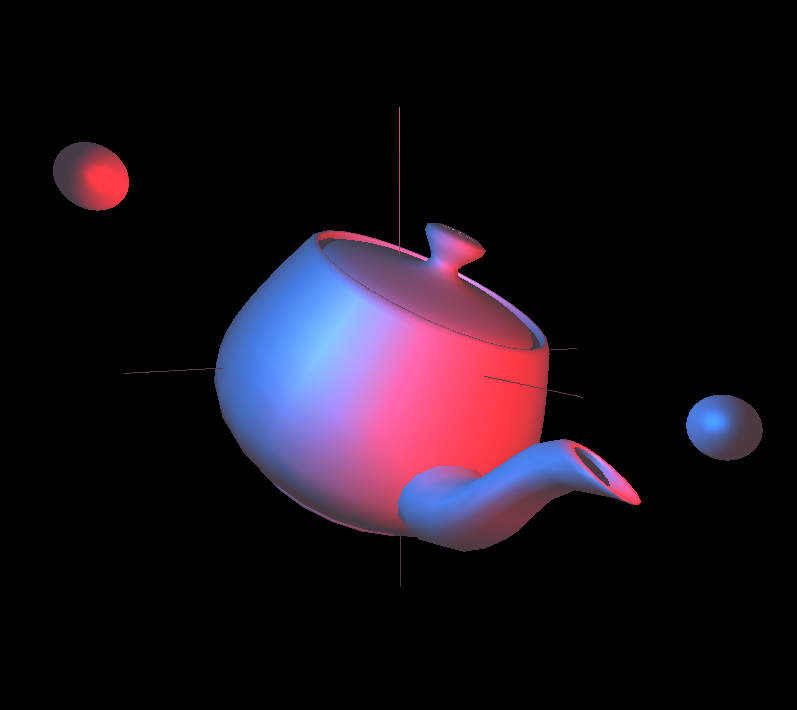
\includegraphics[width=0.55\linewidth, trim={0cm 3cm 0cm 3cm},clip]{img/teapot_1.png}
    \caption{Widok imbryczka z zastosowaną zmianą obrotu i skali modelu, zmianą położenia kamery, oświetlonego dwoma źródłami światła.}
\end{figure}
\begin{figure}[H]
    \centering
    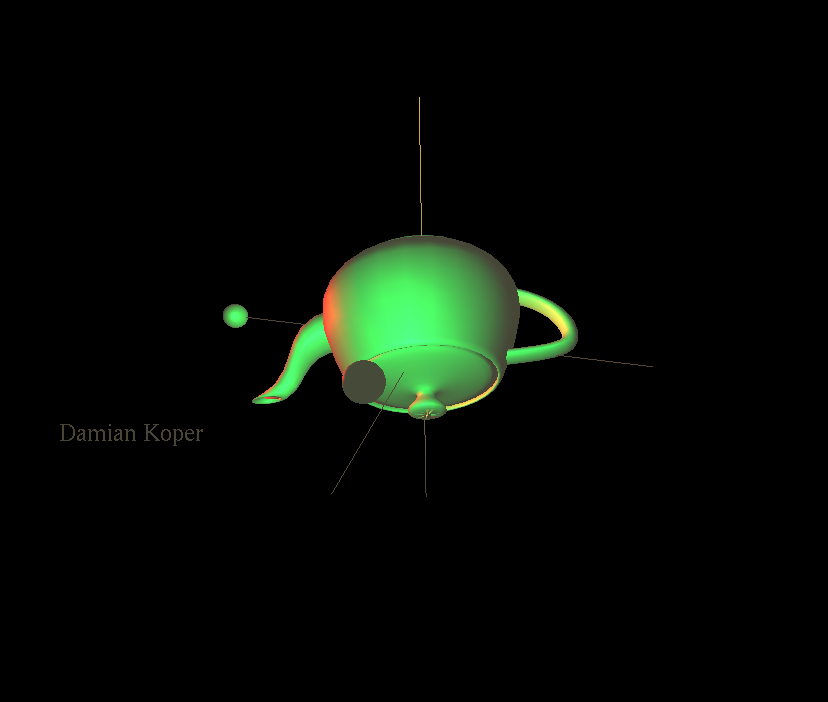
\includegraphics[width=0.8\linewidth, trim={0cm 6cm 0cm 2cm},clip]{img/teapot_2.png}
    \caption{Imbryczek w innej pozycji, widziany z innego punktu. Barwa światła znajdującego się bliżej kamery została zmieniona na zieloną.}
\end{figure}
\subsection{Oświetlenie jajka}
Wokół obracającego się modelu jajka zostały umieszczone dwa orbitujące pod różnym kątem i z różną prędkością źródła światła.
\begin{figure}[H]
    \centering
    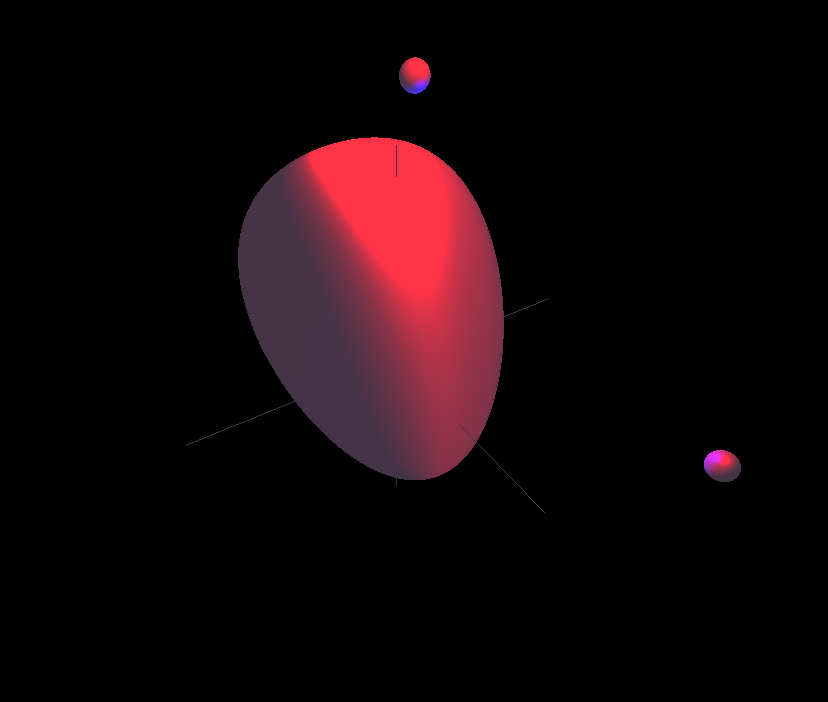
\includegraphics[width=0.8\linewidth, trim={0cm 6cm 0cm 0.5cm},clip]{img/egg_4.png}
    \caption{Oświetlony model jajka.}
\end{figure}